\documentclass[12pt]{article}
\usepackage{cite}
\usepackage{indentfirst}
\usepackage{subcaption}
\usepackage{graphicx}
\title{Volunteer Connector - User Stories and Set-up Assignment}
\author{Daniel Domme (onid: dommed), \\
Charles Koll (onid: kollch), \\
Pedro Autran e Morais (onid: autranep), \\
Coulby Nguyen (onid: nguyenco), \\
Pavel Shonka (onid: shonkap)
}
\date{26 February 2018}

\begin{document}
\maketitle
\tableofcontents

\pagebreak
\section{User Stories and Corresponding Tasks}
\begin{itemize}
\item
	Home page (to be completed by 3/3)

	- User can click on home page and see all posts

	- Should be done first

	- Will take about 2 days to complete
\item
	Event Info (to be completed by 3/9)

	- Organizations can post information about their events

	- Can start after home page and accounts is completed

	- Will take about 2 days to complete
\item
	Volunteer Account (to be completed by 3/3)

	- User account can save their posts

	- Database should be completed before home page can be completed

	- Will take about 2 days to complete
\item
	Charity Accounts (to be completed by 3/3)

	- Only charities can post, edit, and delete posts

	- Can be completed after database is done

	- Will take about 2 days to complete
\item
	Login Button (to be completed by 3/3)

	- User can click a button to input login info

	- Needs to e done before home page is completed

	- Will take about 1 day to complete
\item
	Sign up/Register button (to be completed by 3/3)

	- User can click a button for pop up window

	- Can be done anytime after login button

	- Will take about 2 days to complete
\item
	Filter query (to be completed by 3/9)

	- User can select certain aspects they are looking for and relevant posts will stay

	- Can be started at same time as home page

	- Will take about 3 days to complete
\item
	Looking at 1 specific posting (to be completed by 3/9)

	- User can select a single post, and that post's details are expanded

	- Can be started at same time as home page

	- Will take about 1 day to complete
\item
	Post Information (to be completed by 3/9)

	- Searchable keywords will be included in post information

	- Can be started at same time as home page

	- Will take about 1 day to complete
\item
	Register Pop-Up (to be completed by 3/3)

	- There will be a pop up with form to input information for a new account

	- Can be done at any point after database is done

	- Will take about 2 days to complete
\item
	Volunteer button (to be completed by 3/9)

	- User can input information for organization to see

	- Home page should be done first

	- Will take about 2 days to complete
\item
	Search Distance (to be completed by 3/9)

	- Searching for posts will have a slider bar for distance from a specified location

	- Can be started at same time as home page

	- Will take about 3 days to complete
\item
	Looking at user's signed up events (to be completed by 3/9)

	- User can click on events registered and the listing of the events they signed up for will appear

	- Start after database is complete

	- Will take about 2 days to complete
\item
	Recent Posts (to be completed by 3/9)

	- Recent posts will appear on the front page

	- Start after database is complete

	- Will take about 2 days to complete
\item
	Home button (to be completed by 3/9)

	- User can click the home button to return to the home page

	- Should be done with home page

	- Will take about 1 day to complete
\item
	About (to be completed by 3/9)

	- There will be a tab that explains what the website is for on the side of homepage

	- Done at any time

	- Will take about 1 day to complete
\item
	Other posts (to be completed by 3/9)

	- Non recent posts are compiled into a single list after recent posts

	- Start after database is complete

	- Will take about 3 days to complete
\item
	Login Popup (to be completed by 3/9)

	- There will be a pop up with fields where user can input account information

	- Completed at any time

	- Will take about 2 days to complete
\item
	Organization info (to be completed by 3/9)

	- Each organization's page has an about section on it

	- Completed at any time

	- Will take about 1 day to complete
\item
	User not Found (to be completed by 3/3)

	- There will be a pop up if password or user name is incorrect

	- Can be completed after database is done

	- Will take about 1 day to complete
\end{itemize}
\section{UML Sequence Diagrams}
Home Page
\begin{figure}[h!]
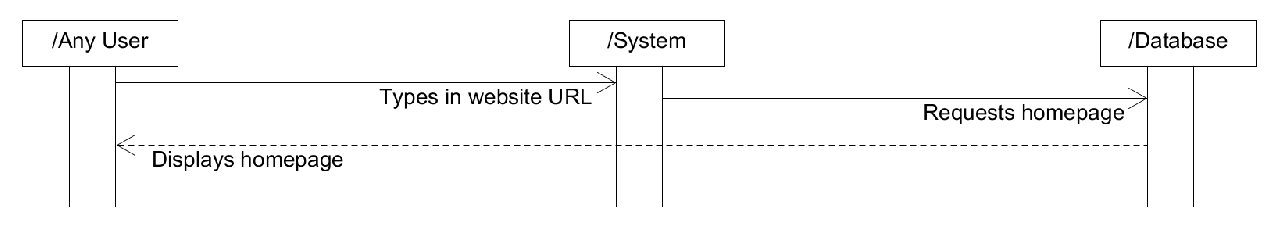
\includegraphics[width=\textwidth]{homepage}
\end{figure}

Volunteer Account
\begin{figure}[h!]
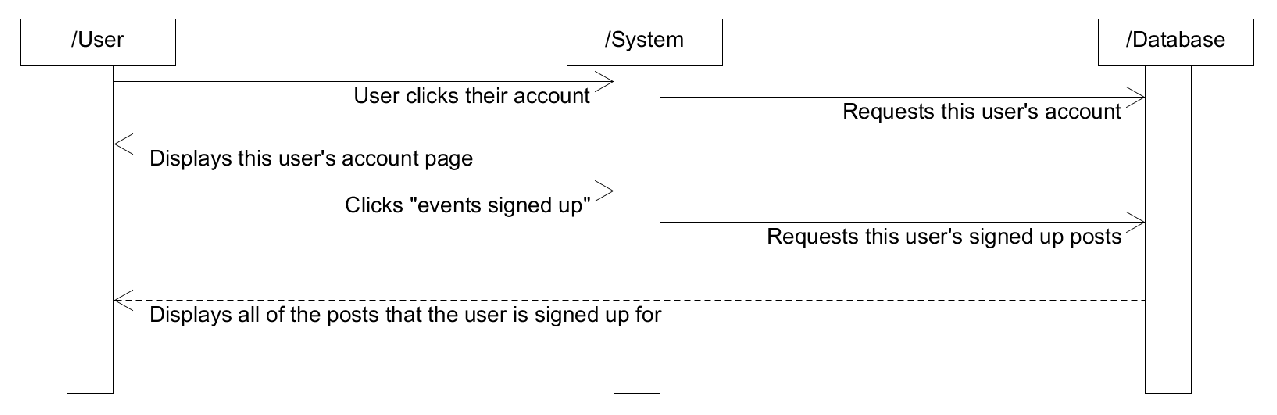
\includegraphics[width=\textwidth]{volunteeraccount}
\end{figure}
\pagebreak

Organization Functionality
\begin{figure}[h!]
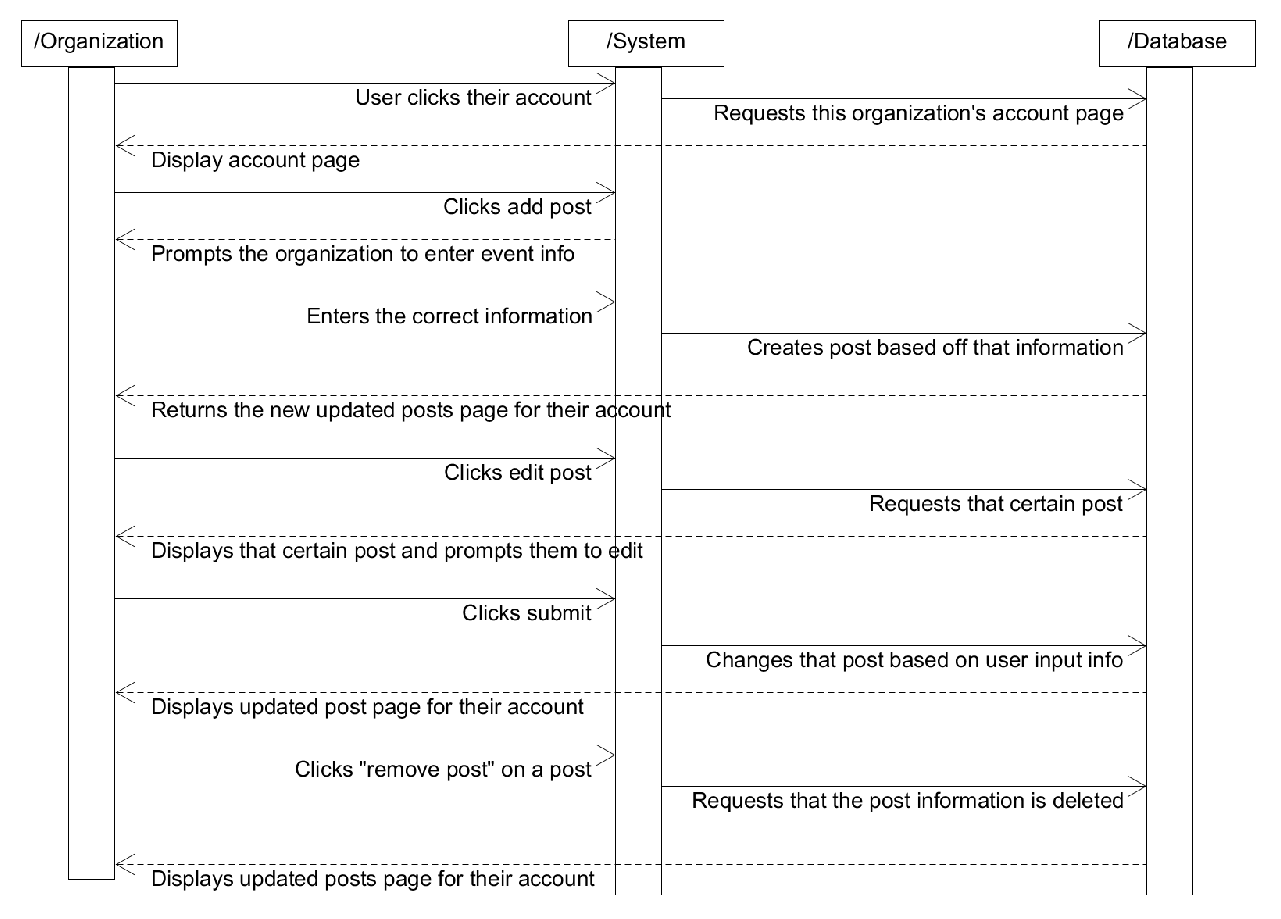
\includegraphics[width=\textwidth]{organizationalfunctionality}
\end{figure}

Login button
\begin{figure}[h!]
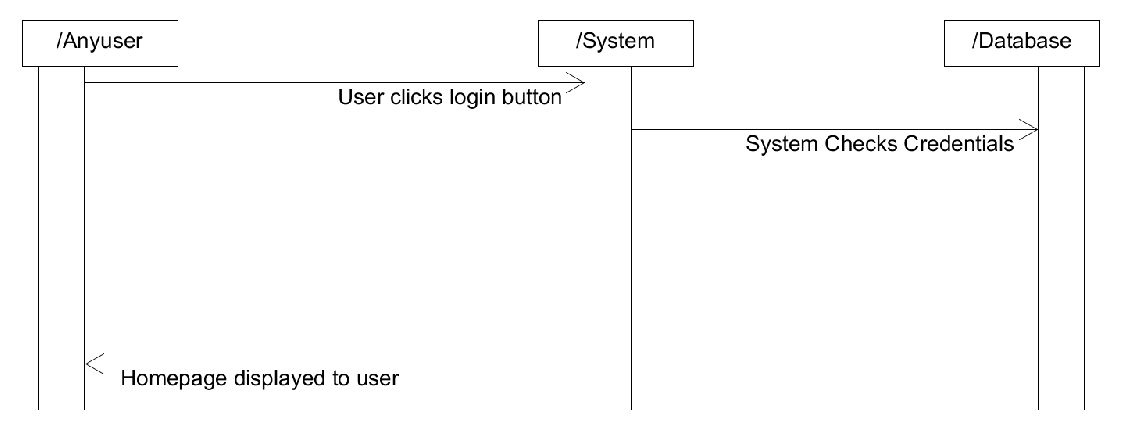
\includegraphics[width=\textwidth]{loginbutton}
\end{figure}
\pagebreak

Register popup
\begin{figure}[h!]
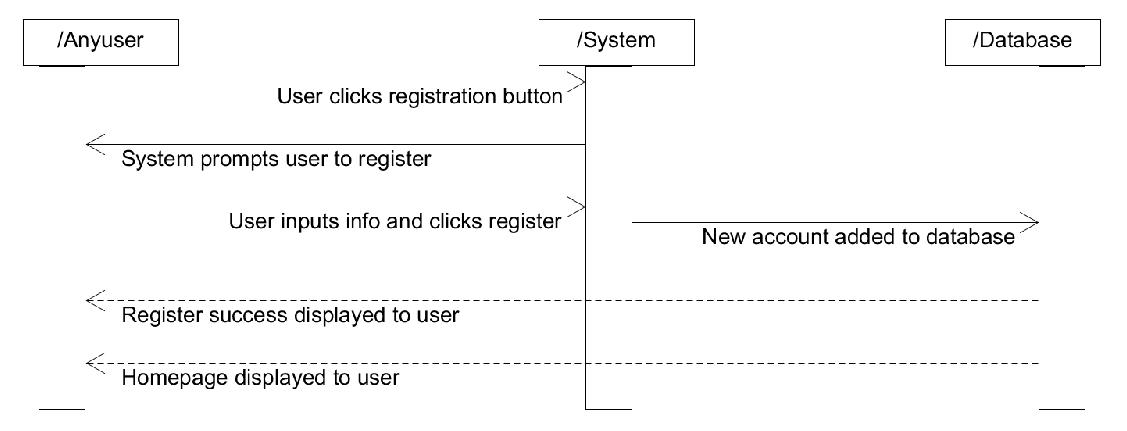
\includegraphics[width=\textwidth]{registerpopup}
\end{figure}

Account not found
\begin{figure}[h!]
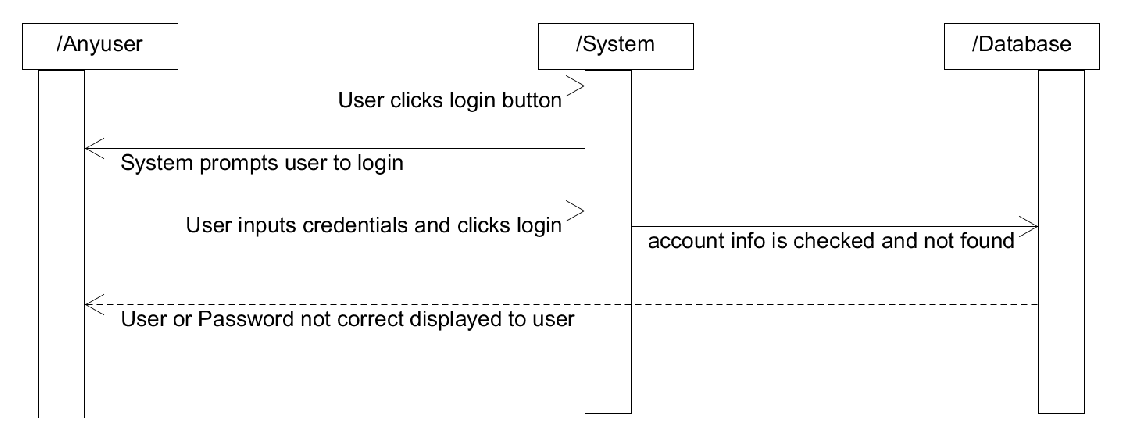
\includegraphics[width=\textwidth]{accountnotfound}
\end{figure}
\section{The Stories due Next Week}
\begin{itemize}
\item
	Coulby, Pavel, Pedro, Charles: Home page will be designed by two members and the
	two others will help connect it to the database

	- Started 3/1
\item
	Coulby, Pavel, Pedro, Charles: Database will be done by Pedro and Charles while
	the actual page and CSS will be done by the other two members

	- Started 3/1
\item
	Pedro, Charles, Daniel: Database will be connected by Pedro and Charles with help
	from Daniel

	- Started 3/1
\item
	Daniel: Pop up that will be designed by one member and implemented into the
	database by the others

	- Started 3/2
\item
	Daniel: Another pop up that will be designed by one member and implemented into
	the database by the others

	- Started 3/2
\item
	Daniel, Pedro, Charles: Little pop up that will be designed by one member and
	connected to database by others

	- Started 3/3
\end{itemize}
\section{Meeting Report}
This week, our group met twice, once on Thursday and once on Sunday, to go plan our
project and complete tasks. We met with the customer and went over user stories. We split
the tasks up between the developers, prioritized sections of the website, and made a
tentative schedule for deadlines for each feature. Sequence diagrams were made for each of
the user stories that we plan on implementing by next week. All of the tasks seem
reasonable, and we should be able to accomplish all tasks in the time allotted.

For next week, we plan on coding some of the basics of the website. This includes the home
page and accounts along with account type functionality. The team plans on meeting on
Monday and Thursday of next week to start coding of the website.

\quad

\subsection{Contributions}
\begin{itemize}
\item
	Daniel Domme: Sequence Diagrams, User Stories
\item
	Charles Koll: User Stories, Latex document compilation
\item
	Pedro Autran e Morais: User Stories, Tasks
\item
	Coulby Nguyen: Sequence Diagrams, User Stories
\item
	Pavel Shonka: User Stories, Implementation
\end{itemize}
\end{document}
